
\chapter{Statistics tests (non-parametric)}
\label{chap:statistics-tests-non}

\section{Paired-t test (Wilcoxon signed-rank test)}
\label{sec:paired-t-test-1}

This is an analog to paired t-test but applied to non-parametric
approach. 


\begin{lstlisting}
library(stats)

wilcox.test(x, y = NULL, 
    alternative = c("two.sided", "less", "greater"), 
    mu = 0, paired = FALSE, exact = NULL, 
    correct = TRUE,
    conf.int = FALSE, conf.level = 0.95,...)
\end{lstlisting}

\section{Logrank test (Mantel-Cox test): in clincal trials}

When the data are right skewed and censored, we use log-rank test (or Mantel-Cox
test, or time stratified Cochran-Mantel-Haenszel test).
It's widely used in clinical trial to compared the efficiency of new treatment
vs. control when the measurement is the time to event (e.g. time from initial
treatment to a heart attack). Log-rank test can be applied for 2 groups or more.

\begin{framed}
The test was proposed by Mantel, and named {\it logrank} by Richard \& Peto
\end{framed}


The variable of interest is {\it time until the event to occur}. So time here is
survival time, and the event is a failure. The censoring means that we don't
know survival time exactly, Fig.\ref{fig:logrank_info}. Let define $T$=failure
time with distribution $F$ (density $f$), $C$=censoring time with distribution
$G$ (density $g$). We assume $C$ and $T$ are independent. The two survival
curves from 2 groups can be drawn using {\bf Kaplan-Meier survival curves}. The
null hypothesis H$_o$: no difference between (true) survival curves. The
log-rank statistics for 2 groups:
\begin{equation}
\frac{\left(O_2-E_2\right)^2 }{\text{Var}\left(O_2-E_2\right) } \approx \chi^2_1
\end{equation}

\begin{figure}[hbt]
  \centerline{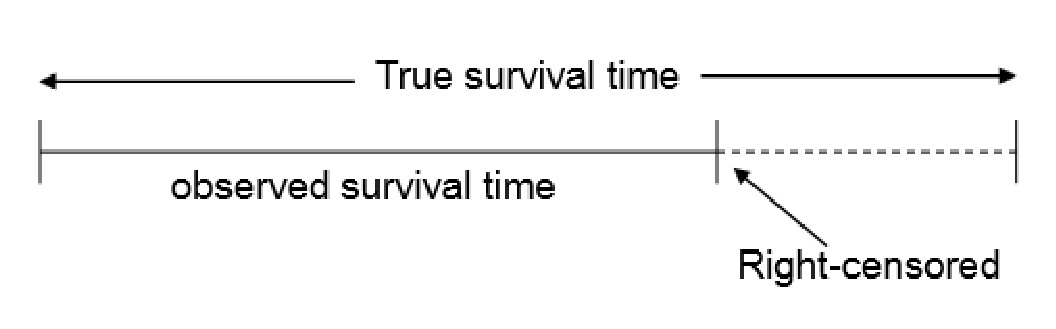
\includegraphics[height=2cm,
    angle=0]{./images/logrank_info.eps}}
  \caption{Log-rank test}
\label{fig:logrank_info}
\end{figure}

R code: \verb!survdiff! function
\begin{verbatim}
time <-c(6,6,6,7,10,13,16,22,23,6,9,10,11,17,19,20,25,32,32,34,35,1,1,2,2,3,4,4,5,5,8,8,8,8,11,11,
12,12,15,17,22,23)
status <-c(1,1,1,1,1,1,1,1,1,0,0,0,0,0,0,0,0,0,0,0,0,1,1,1,1,1,1,1,1,1,1,1,1,1,1,1,1,1,1,1,1,1)

treatment <-c(1,1,1,1,1,1,1,1,1,1,1,1,1,1,1,1,1,1,1,1,1,2,2,2,2,2,2,2,2,2,2,2,2,2,2,2,2,2,2,2,2,2)
fit <-survdiff(Surv(time, status) ~ treatment)
\end{verbatim}
The result
\begin{verbatim}
fit
Call: survdiff(formula = Surv(time, status) ~ treatment)
            N   Observed Expected (O-E)^2/E (O-E)^2/V
treatment=1 21  9        19.3     5.46      16.8
treatment=2 21  21       10.7     9.77      16.8

Chisq = 16.8 on 1 degrees of freedom, p = 4.17e-05
\end{verbatim}
In this example, the test is significant to reject H$_o$ (as the chance to
observe H$_o$ is too small).

Alternative methods (derived by applying different weights at the $j$-th
failure time, Fig.\ref{fig:logrank_weight}): Wilcoxen, Tarone-Ware, Peto,
Flemington-Harrington. So the question is \textcolor{red}{Which test to use?}: 
\begin{enumerate}
  \item The best choice is test with most power
  \item There may be a clinical reason to choose a particular weighting
  \item Choice of weight should be a priori (not fish for a desire p-value)
  \item Using different weights should usually give the same conclusion
\end{enumerate}

\begin{figure}[hbt]
  \centerline{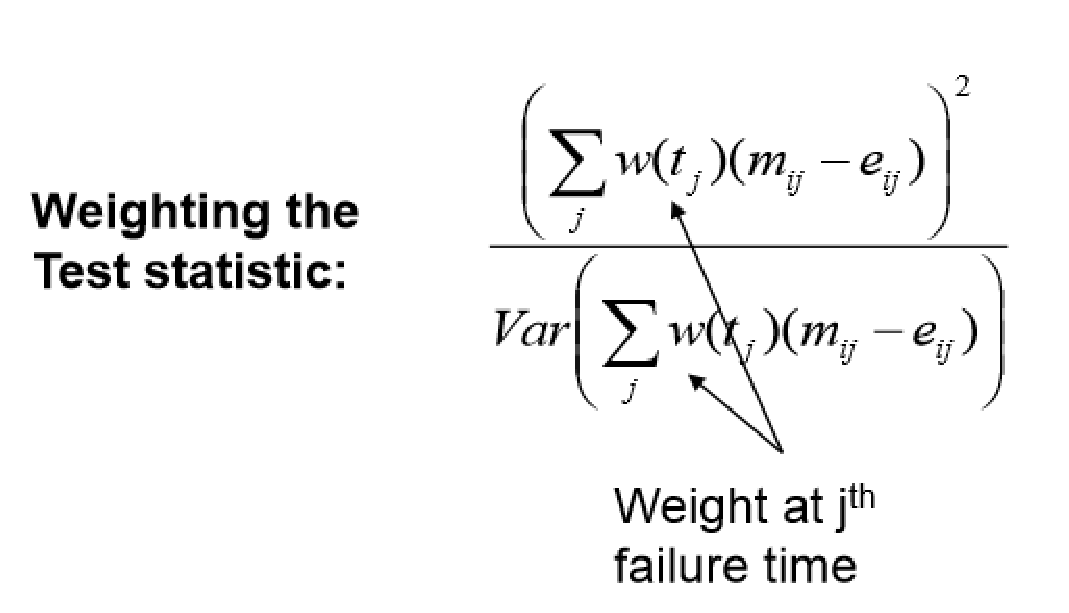
\includegraphics[height=3cm,
    angle=0]{./images/logrank_weight.eps}}
  \caption{Alternative to Log-rank test using weights}
\label{fig:logrank_weight}
\end{figure}

\url{http://stat.ethz.ch/education/semesters/ss2011/seminar/contents/presentation_2.pdf}

\subsection{Stratified logrank test}

When there is additional 'stratified' variable, data can be splitted based on
the value of stratified variable. In stratified logrank test, the data are
groupped into strata, Fig.\ref{fig:logrank_stratified}. So, $(O-E)$ are
calculated based on data within strata, and sum $(O-E)$ across strata. The
limitation is that sample size may be small with strata.


\begin{figure}[hbt]
  \centerline{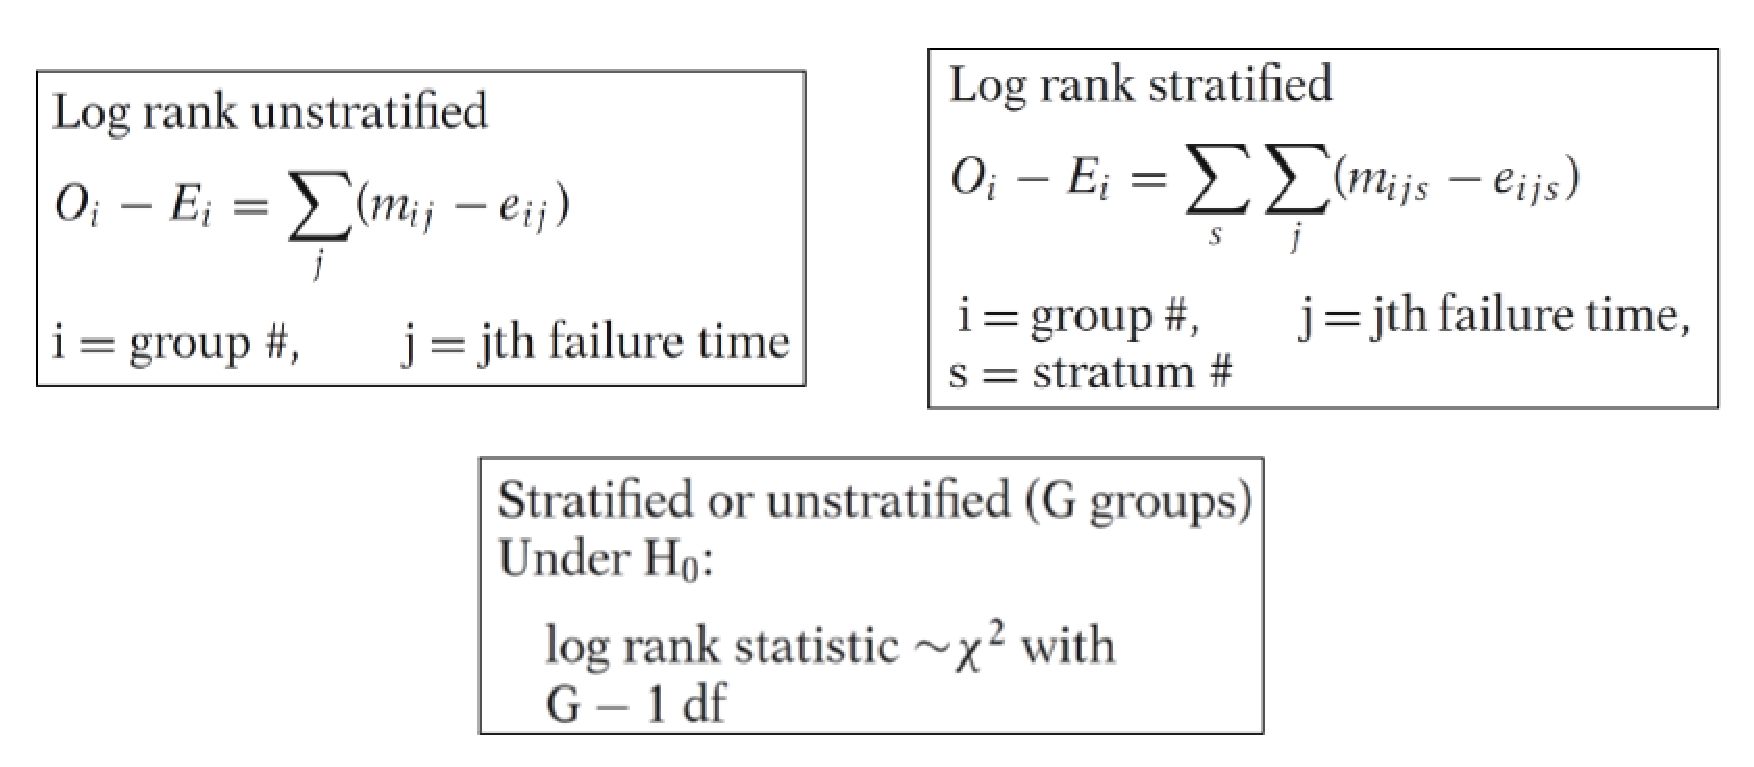
\includegraphics[height=3cm,
    angle=0]{./images/logrank_stratified.eps}}
  \caption{Comparison between stratified vs. unstratified logrank tests}
\label{fig:logrank_stratified}
\end{figure}


R code
\begin{verbatim}
data<-read.table("http://www.sph.emory.edu/~dkleinb/surv2datasets/anderson.dat")
lwbc3<-c(1,1,1,2,1,2,2,1,1,1,3,2,2,2,2,2,3,3,2,3,3,1,2,2,1,1,3,3,1,3,3,2,3,3,3,3,2,3,3,3,2,3)

fit <-survdiff(Surv(data$V1,data$V2)~data$V5+strata(lwbc3))
\end{verbatim}
The result is
\begin{verbatim}
fit 
Call: survdiff(formula = Surv(data$V1,data$V2)~ data$V5 + strata(lwbc3))

           N Observed Expected (O-E)^2/E (O-E)^2/V
data$V5=0 21 9        16.4      3.33      10.1
data$V5=1 21 21       13.6      4.00      10.1

Chisq =10.1 on 1 degrees of freedom,p =0.00145
\end{verbatim}

%%% Local Variables: 
%%% mode: latex
%%% TeX-master: "R_language"
%%% End: 
